% !TeX root = ../praktikum.tex
% !TeX encoding = UTF-8
% !Tex spellcheck = de_DE

In diesem Versuchsabschnitt wurden die Längs- und Querspannung gemessen und aufgezeichnet, während an der Probe ein Gleichstrom anlag. Gleichzeitig wurde das Magnetfeld verändert.

Um eine stabile Temperatur zu erhalten, wurde die Kammer von den \unit[1,5]{K} auf \unit[2]{K} geheizt und programmgesteuert auf dieser Temperatur gehalten. Der Strom in x-Richtung betrug $\unit[1]{\mu A}$. Das Magnetfeld wurde auf \unit[-7,7]{T} gefahren. Dies dauert rund sieben Minuten, da es sich um supraleitende Spulen handelt und das Anlegen eines Stroms eine Gegeninduktion verursacht. Sobald das Magnetfeld aufgebaut war, wurde die Hallspannung $U_H$ sowie die Längsspannung $U_{xx}$ aufgezeichnet, während das Magnetfeld mit der maximalen Geschwindigkeit von \unitfrac[1]{T}{min} auf \unit[+7,7]{T} gefahren wurde.\\

Die mit Hilfe der Formeln~\eqref{eq:rho_xx} und \eqref{eq:rho_xy} aus den Spannungen berechneten Widerstände sind in Abbildung~\ref{fig:full_range_dc} zu sehen.

\begin{figure}[h]
	\centering
	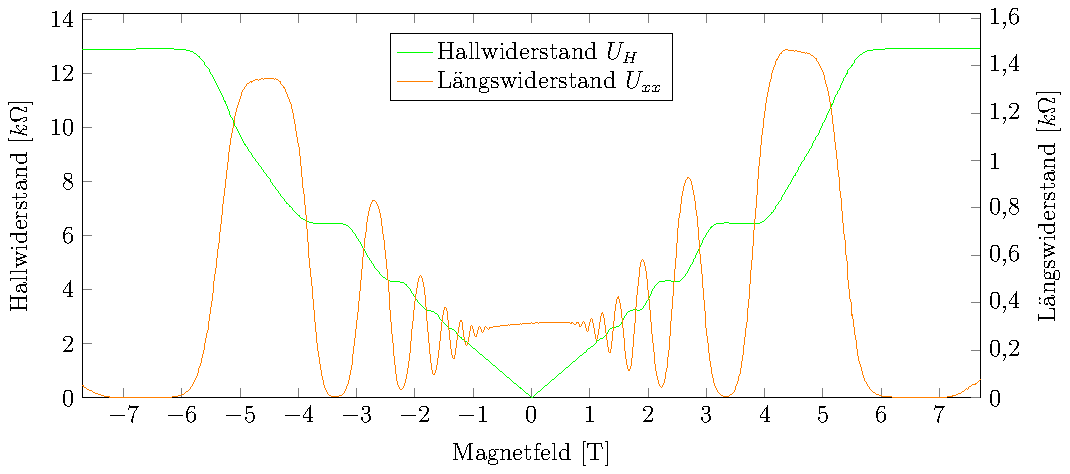
\includegraphics[scale=1]{graphs/dc/full_range.pdf}
	\caption[Gleichstrommessung im maximalen Magnetfeldbereich]{
		Plot des aus den gemessenen Längs- und Querspannungen berechneten Widerständen eines mit Gleichstrom durchflossenen 2DES im maximalen Magnetfeldbereich und maximaler Magnetfeldrampe. Die Hall-Spannung und somit der berechnete Hall-Widerstand nimmt bei negativen Magnetfeldern negative Werte an, Aus Platzgründen wurde diese jedoch in den positiven Bereich geklappt.
	}
	\label{fig:full_range_dc}
\end{figure}

Um im Bereich von $-2$ bis \unit[+2]{T} eine bessere Auflösung der sehr dicht beieinander liegenden Niveaus zu bekommen wurde eine zweite analoge Messung in diesem Bereich mit einer kleineren Magnetfeldrampe von \unitfrac[0,2]{T}{min} durchgeführt. Da das Fahren der Magnetfelder, wie bereits erwähnt, längere Zeiten in Anspruch nimmt, kann hier mit vorausschauendem Handeln viel Zeit gespart werden. Daher wurde das Magnetfeld von den \unit[+7,7]{T} aus dem letzten Versuchsteil erst auf \unit[+2,2]{T} gefahren und die Messung anschließend mit einer negativen Magnetfeldrampe durchgeführt.

Die aus den Messergebnissen berechneten Widerstandsverläufe sind in Abbildung~\ref{fig:2T_range_dc} aufgetragen.\\

\begin{figure}[h]
	\centering
	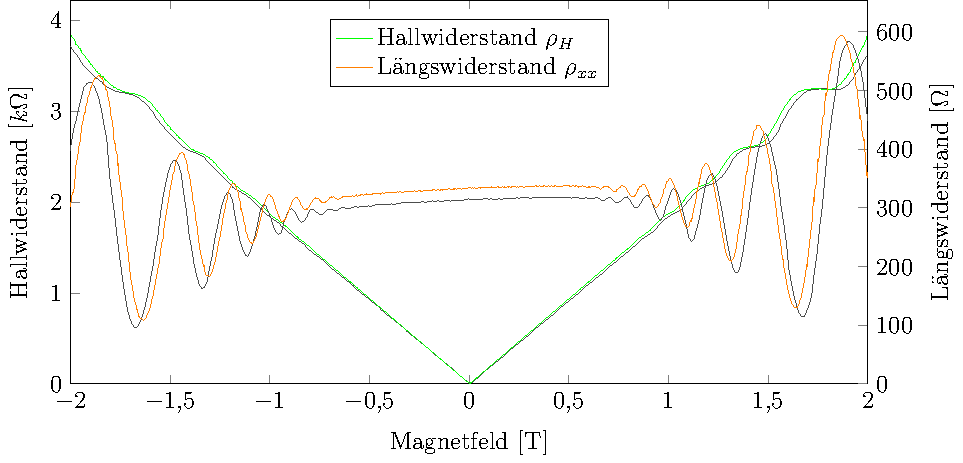
\includegraphics{graphs/dc/pm2T_range.pdf}
	\caption[Höher aufgelöste Gleichstrommessung in Magnetfeldteilbereich]{
		Plot des aus den gemessenen Längs- und Querspannungen berechneten Widerständen eines mit Gleichstrom durchflossenen 2DES im reduzierten Magnetfeldbereich und geringerer Magnetfeldrampe. Die Hall-Spannung und somit der berechnete Hall-Widerstand nimmt bei negativen Magnetfeldern negative Werte an, Aus Platzgründen wurde diese jedoch in den positiven Bereich geklappt.
	}
	\label{fig:2T_range_dc}
\end{figure}


Es sind deutlich die Plateaus des Hall-Widerstandes und die Oszillation des Shubnikov-de Haas-Widerstandes zu erkennen. Die Maxima der SDHO liegen bei den Übergängen zwischen den Plateaus des QHE. Ferner ist eine leichte Asymmetrie der Messergebnisse zwischen positiven und negativen Magnetfeldern zu erkennen. 